% !TEX encoding = UTF-8 Unicode
%!TEX root = ../Main/thesis.tex
% !TEX spellcheck = en-US
%%=========================================
\documentclass[../Main/thesis.tex]{subfiles}
\begin{document}
\chapter{First Iteration  - Establishing requirements}
\label{ch:requirements}
This chapter describes the first step in the development process: establishing requirements for the system. 

\section{Initial requirements}
The first requirements that were established was the overall structure of the system and which technologies should be used.
It was decided that BLE should be used as the technology for localization.
The data from the BLE beacons should be collected using cellphones, running the Android operation system, attached to the smoke divers.
This data should then be visualized in a web interface.

The initial requirements was then:
An Android application that could track the Bluetooth signal from the beacons and upload them to a server.
A back-end that could receive data from the cellphone, process the raw data and present it through a REST API.
A web-application for presenting and visualizing the processed data from the back-end.

\subsection{Android Application}
Before the initial meeting with Øygarden Fire and Rescue (ØFR) a design-prototype of the Android application was created. 
This purpose of this prototype was to showcase both a suggestion of how the application would be used, and, most important, how the app should function.
The first step in creating the prototype was to create the flowchart shown in Figure~\ref{fig:flow-app-1}, visualizing user actions in the app.

\begin{figure}
	\centering
	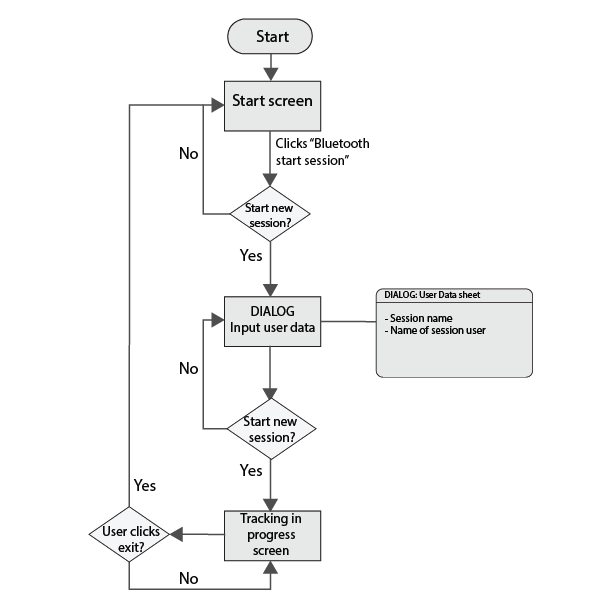
\includegraphics[width=0.6\linewidth]{../fig/flow_wire_app_1}
	\caption{Flowchart of the Android application}
	\label{fig:flow-app-1}
\end{figure}

As the application only have one feature, it should be as simple as possible. 
The user of the application should be able to create a new session with a name and a user and start the session. 
Then the application should collect data from nearby BLE devices until the user end the session.
The application should then upload the collected data to the server for processing.

When the initial requirements was included in the flowchart a wireframe was created as shown in Figure~\ref{fig:wireframe-app-1}.
This was created both to present a possible design, and to present how the app could be used to the firefighters. 

\begin{figure}
	\centering
	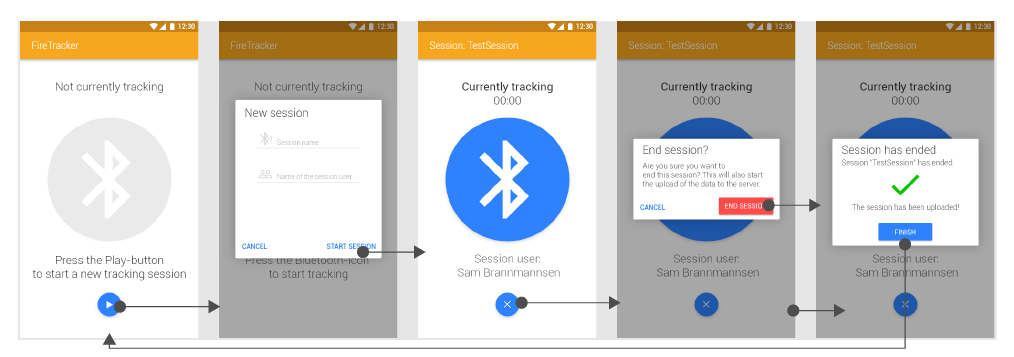
\includegraphics[width=\linewidth]{../fig/wireframe_app_1}
	\caption{Wireframe of the Android application}
	\label{fig:wireframe-app-1}
\end{figure}

\subsection{Back-end}
At this stage the only defined requirements for the back-end was that it should be able to receive data through a REST API, process the data, and present it through a REST API.

\section{Input from the fire department}
The requirements established this far was based on previous experience with development and an idea of how this system could be used, and what the fire department needed.
To better understand what they actually need, and how they think they can use the system, an interview with the fire chief and one of the instructors was conducted.
The interview session started with an observation of a smoke diving exercise and was then followed by the actual interview, which can be divided into three main parts: practical aspects, visualization and presentation of data, and use of data.

\subsection{Practical questions}

\subsection{Visualization questions}

\subsection{Using the data}



\end{document}
